\section{Supercompilation by Example}
\epigraph{The advantages of every formal language are determined not only
by its ease of use by humans, but also by the amenability of its texts to 
formal transformations.}{V.F. Turchin \cite{Turchin1974EqTrans}}

It would be nice if all computer-science articles were accompanied by some formal 
executable description (in the form of a program or a formal specification)
in order to ensure reproducibility of results.

The SC~Mini supercompiler is such an executable description of the fundamental 
methods of supercompilation, which are the main topic of this article.
SC~Mini is based on the supercompiler described in the groundbreaking
MSc thesis of Morten H. S{\o}rensen
\cite{Sorensen1994TurchinSupercompiler} 
(which remained only on paper).

No supercompilation description is complete without describing subtle fundamental notions
such as program semantics, evaluation results, computation state. 
All these notions are formally represented in the sources of SC~Mini, which helps
avoid ambiguities.

SC~Mini transforms programs written in a toy language called SLL
(= Simple Lazy Language; corresponding roughly to 
S{\o}rensen's $M_0$).
Paraphrasing Turchin's quote from the beginning of the section, we argue
that SLL's main advantages are:
\begin{enumerate}
  \item A simple language definition, and
  \item A simple definition of a supercompiler for SLL programs.
\end{enumerate}

Despite the fact that SC~Mini is a supercompiler for a specific language, the methods used 
in its construction are fairly general and appear with only small variations in most supercompilers.

We shall see further through several examples that SC~Mini can optimize programs 
(giving first a formal definition of a program optimizer),
and it can also be used to automatically prove different program properties.

%The article contains some small-print remarks, which can be safely skipped
%or only skimmed on first reading, but it is worth returning to them
%after becoming acquainted with SC~Mini's sources.
%The purpose of these remarks is to highlight some important subtleties
%concerning the correctness of the performed transformations.
%It is such subtleties that make supercompiler writing a difficult art.
%
%We next formally introduce the SLL language.

\subsection{SLL Object Language}
\label{sec-formalities}

\begin{figure}[t!]
\caption{SLL abstract syntax}
\begin{tabular}[t]{l r l@{\hspace{20pt}} l}
$P$ & ::=    & $d_1 \ldots d_n$                  & program   \\
\\
$d$ & ::=    &  $f(v_1, \ldots, v_n) = e;$       & ``indifferent'' function \\
    & $\mid$ & $g(p_1, v_1, \ldots, v_n) = e_1;$ & ``curious'' function \\
    &        & $\ldots$ \\
    &        & $g(p_m, v_1, \ldots, v_n) = e_m;$ \\
\\
$e$ & ::= && expression  \\
    && $v$                    &variable\\
    &$\mid$  & $C(e_1, \ldots, e_n)$  &constructor\\
    &$\mid$  & $f(e_1, \ldots, e_n)$  &function call\\
\\
$p$ & ::=    & $C(v_1, \ldots, v_n)$  &pattern
\end{tabular}
\label{fig-sll-syntax}
\end{figure}

\begin{figure}[t!]
\caption{\texttt{prog1}: Working with Peano numbers}
\label{fig:prog1}
\begin{lstlisting}[language=sll]
add(Z(), y)  = y;
add(S(x), y) = S(add(x), y);

mult(Z(), y)  = Z();
mult(S(x), y) = add(y, mult(x, y));

sqr(x) = mult(x, x);

even(Z())  = True();
even(S(x)) = odd(x);

odd(Z())  = False();
odd(S(x)) = even(x);

add'(Z(), y)  = y;
add'(S(v), y) = add'(v, S(y));
\end{lstlisting}
\end{figure}

Defining a language entails defining its syntax and semantics. 
Syntax is typically defined using a context-free grammar.
One possible way to define semantics is to implement an interpreter for the language.
The following natural-language description is more succinctly and simply 
re-expressed -- using Haskell -- in SC~Mini's sources.

%\subsubsection{Syntax} 
Fig.~\ref{fig-sll-syntax} gives the abstract syntax of SLL.
An SLL expression can be one of the following:
\begin{itemize}
  \item variable,
  \item constructor, having SLL expressions as arguments, or a
  \item function call, having SLL expressions as arguments.
\end{itemize}

We assume further the same convention as in Haskell: constructor names start
with an uppercase letter; variable names start with a lowercase letter.

An SLL expression consisting only of constructors is called a \emph{value}.
An SLL expression without any variables inside is called a \emph{closed expression}.
We define \emph{configuration} as an alias of an SLL expression with free variables.

An SLL program consists of function definitions.
We distinguish two kinds of functions -- ``indifferent'' and ``curious''
(originally called by S{\o}rensen in \cite{Sorensen1994TurchinSupercompiler} f- and g-functions respectively).
Curious functions replace case expressions (which are always lifted to the top level).
%and remove the need to deal with nested bound variables.
Indifferent functions just transfer their arguments to other functions or constructors;
their definition is just a single expression.
Curious functions perform a simple pattern match on their first argument;
their definitions consist of many expressions -- one per case.

SLL has no built-in data types (Booleans, numbers, etc.). 
SLL can be straightforwardly extended with Haskell-like data-type
declarations and Hindley-Milner type inference, but we ignore
issues of typing from now on, silently assuming that all
programs under consideration would be well-typed
under such a type system.
We assume the following convention:
\begin{itemize}
  \item the constructors \texttt{True()} and \texttt{False()} represent Boolean values,
  \item the value \texttt{Z()} represents $0$, \texttt{S(Z())} - $1$, \texttt{S(S(Z()))} - $2$, etc. 
    If the value \texttt{n} corresponds to the natural number $n$, then the value \texttt{S(n)}
	corresponds to the natural number $n+1$ (the so-called Peano numbers).
\end{itemize}

Fig.~\ref{fig:prog1} shows a program defining some functions for working
with Peano numbers.
It contains a single indifferent function -- squaring (\texttt{sqr}).
All the other functions are curious, as they do a pattern match on their first argument.

A \emph{substitution} binds variables $v_1, v_2, \ldots, v_n$ to expressions $e_1, e_2, \ldots, e_n$ 
and is written as a list of pairs $\{v_1:=e_1, \ldots, v_n := e_n\}$.
Application of a substitution to an expression $e$ is defined in the usual way, and 
is denoted $e / \{v_1:=e_, \ldots, v_n := e_n\}$.

\begin{exercise}
In SC~Mini's sources substitution is literally represented as a list of pairs.
Application of a substitution \texttt{s} to an expression \texttt{e} is denoted as \texttt{e~//~s}.
Find \texttt{e}, \texttt{v1}, \texttt{e1}, \texttt{v2}, \texttt{e2}, such that
\\ \texttt{e // [(v1, e1), (v2, e2)]} $\not =$ \texttt{e // [(v1, e1)] // [(v2, e2)]}.
\end{exercise}

% и этот тоже
%\subsubsection{Semantics}

\begin{figure}[t!]
\caption{SLL: interpreter $\mathcal{I}_p$ for a program $p$}
\begin{tabular}{@{}l@{\hspace{1pt}} l@{\hspace{1pt}} l@{\hspace{1pt}} l@{\hspace{1pt}}}
$\mathcal{I}_p \llbracket e \rrbracket$ &
$\Rightarrow$
$e$ & ($I_1$)\\&if $e$ is a value\\

$\mathcal{I}_p \llbracket C(e_1, \ldots, e_n) \rrbracket$ &
$\Rightarrow$
$C(\mathcal{I}_p \llbracket e_1 \rrbracket, \ldots, \mathcal{I}_p \llbracket e_n \rrbracket)$ & ($I_2$) \\ \\

$\mathcal{I}_p \llbracket con \langle f(e_1, \ldots, e_n) \rangle \rrbracket$ &
$\Rightarrow$
$\mathcal{I}_p \llbracket con \langle e / \{v_1 := e_1, \ldots, v_n := e_n\} \rangle \rrbracket$ & ($I_3$) \\
&if $f(v_1, \ldots, v_n) \stackrel{\textrm{\tiny p}}{=} e$\\

$\mathcal{I}_p \llbracket con \langle g(C(e_1, \ldots, e_m), e_{m+1},\ldots, e_n)\rangle \rrbracket$ &
$\Rightarrow$
$\mathcal{I}_p \llbracket con \langle e / \{v_1 := e_1, \ldots, v_n := e_n\} \rangle \rrbracket$ & ($I_4$)\\
&if $g(C(v_1, \ldots, v_m), v_{m+1},\ldots, v_n) \stackrel{\textrm{\tiny p}}{=} e$
\end{tabular}
\label{fig-sll-semantics}
\end{figure}

\begin{figure}[t!]
\caption{SLL: context and redex}
\begin{tabular}[t]{l r l@{\hspace{20pt}} l}
$con$ & ::= & $\langle\rangle$
			$\mid$ $g(con, \ldots)$ &context \\
$red$ & ::= & $f(e_1, \ldots, e_n)$
			$\mid$ $g(C(e_1, \ldots, e_n), \ldots)$ &redex
\end{tabular}
\label{fig-sll-context}
\end{figure}

Fig.~\ref{fig-sll-semantics} shows the formal reduction semantics of SLL expressions.
The notation $e_1 \stackrel{\textrm{\tiny p}}{=} e_2$ means that the program $p$ contains a definition $e_1 = e_2$.
The semantics is defined through a rewriting SLL interpreter with normal-order reduction.
The SLL interpreter $\mathcal{I}_p$ processing a program $p$ evaluates, step by step,
each closed SLL expression to an SLL value (or falls into an infinite loop,
or terminates with an error message, but we shall often ignore the last case for simplicity).
As far as reduction is concerned, we distinguish two kinds of closed expressions:
\begin{enumerate}
  \item $e = C(e_1, \ldots, c_n)$ -- a constructor is ``pushed'' outside, and we 
  proceed to reduce its arguments.
  \item $e \not = C(e_1, \ldots, c_n)$ -- then we locate the leftmost reducible function call
  (\emph{redex}, see Fig.~\ref{fig-sll-context}) and unfold it according to
  the corresponding definition from the program.
  A function call is reducible if it is a call to
  1) an indifferent function or
  2) a curious function, where the first argument starts with a constructor.
\end{enumerate}


% Шаг интерпретатора~--- однозначная
% редукция вызова функции. Вызов функции может быть однозначно редуцирован, если это вызов f-функции
% или вызов g-функции с конструктором на месте первого аргумента. SLL-интерпретатор всегда редуцирует
% самый левый вызов, заменяя вызов функции на правую часть определения, подставляя
% соответствующие выражения на место параметров\footnote{Формально семантика SLL определяется как
% система редукций (дана в приложении) с левосторонней (leftmost outermost) редукционной
% стратегией.
% Системы редукций как средство описания операционной семантики разбираются, например, в
% \cite{Mitchell1996Foundations}.}.

The rules for evaluating SLL expressions are (as typical for functional languages) \emph{compositional},
meaning that, if the expression $e_1 / \{v := e_2\}$ is closed, then
(taking laziness into account):
\[\mathcal{I}_p\llbracket e_1 / \{v := e_2\}\rrbracket = \mathcal{I}_p \llbracket e_1 / \{v := \mathcal{I}_p\llbracket e_2\rrbracket\} \rrbracket\]

Remark that we can consider $\mathcal{I}_p$ as a machine, describing the program $p$.

\begin{exercise}
In SC~Mini the interpreter is defined as a function \texttt{eval}.
The notation $\mathcal{I}_p\llbracket e \rrbracket$ corresponds to the call \texttt{eval p e}.
Prove that the evaluation of
\\
\texttt{eval p (e1 // [(v, e2)]) == eval p (e1 // [(v, eval p e2)])}
\\
cannot give \texttt{False}.
\end{exercise}

We call an \emph{SLL-task}
%\footnote{The notion of a SLL-task is introduced to simplify the following descriptions,
%and is analogous to the function \texttt{main} in many programming languages.}
(or sometimes simply \emph{task}) the pair $(e, p)$
of a configuration $e$ and a program $p$
(recall that a configuration is simply an expression with free variables). 
The evaluation of a task $(e, p)$ on arguments $args$ is defined as:
\[\mathcal{R}_{(e, p)}\llbracket args\rrbracket = \mathcal{I}_p\llbracket e / args\rrbracket\]
(In SC~Mini the corresponding call is \texttt{sll\_run (e, p) args}.)

% Стоимость вычисления замкнутого выражения $e$ для программы $p$ -- количество шагов интерпретатора
% при вычислении $\mathcal{I}_p |[e|]$.

Fig.~\ref{fig-sll-int} shows an example of evaluating the expression \texttt{even(sqr(S(Z())))} 
with the interpreter for the program \texttt{prog1}.
The redexes are underlined.
The root node represents the task with its arguments.

\begin{figure}[t!]
\caption{An example of a task evaluation}
\label{fig-sll-int}
\begin{tikzpicture}[
level distance=10mm,
level/.style={sibling distance=45mm},
conf/.style={
	rectangle,minimum width=20mm,minimum height=6mm,rounded corners=3mm,
	draw=black,
	font=\ttfamily\small}, 
system/.style={
	rectangle split, rectangle split parts=2, draw,
	draw=black,fill=black!10,
	font=\ttfamily\small}, 
label/.style={
font=\ttfamily\small
}
]
\tikzstyle{level 1}=[level distance=12mm];
\tikzstyle{level 2}=[level distance=10mm]
\node[system]{(even(sqr(S(x))), prog1) \nodepart{second}x := Z()}
child {node[conf](s0) {even(\underline{sqr}(S(Z())))}
	child[->] {node[conf](s1) {even(\underline{mult}(S(Z()), S(Z())))} 
		child[->] {node[conf](s2) {even(\underline{add}(S(Z()), mult(Z(), S(Z()))))}
			child[->] {node[conf](s3) {\underline{even}(S(add(Z(), mult(Z(), S(Z())))))}
				child[->] {node[conf](s4) {odd(\underline{add}(Z(), mult(Z(), S(Z()))))}
					child[->] {node[conf](s5) {odd(\underline{mult}(Z(), S(Z())))}
						child[->] {node[conf](s6) {\underline{odd}(Z())}
							child[->] {node[conf](s7) {False()}}}}}}}}};
\node[label,right] at ($ (s0.east) + (10mm,0mm) $) {s0};
\node[label,right] at ($ (s1.east) + (10mm,0mm) $) {s1};
\node[label,right] at ($ (s2.east) + (10mm,0mm) $) {s2};
\node[label,right] at ($ (s3.east) + (10mm,0mm) $) {s3};
\node[label,right] at ($ (s4.east) + (10mm,0mm) $) {s4};
\node[label,right] at ($ (s5.east) + (10mm,0mm) $) {s5};
\node[label,right] at ($ (s6.east) + (10mm,0mm) $) {s6};
\node[label,right] at ($ (s7.east) + (10mm,0mm) $) {s7};
\end{tikzpicture}
\end{figure}

%\subsubsection{Optimizer} 
Next, we formally define what is an \emph{optimizer} of SLL tasks.
An SLL optimizer takes a task $(e, p)$ as input and outputs another task $(e', p')$.
Our first requirement is correctness:
for all arguments $args$, the results of both tasks must be the same:
%\footnote{
%Meaning that the SLL interpreter either gives equal results for both tasks, or
%it goes into an infinite loop in both cases.}
\[\mathcal{R}_{(e, p)}\llbracket args\rrbracket = \mathcal{R}_{(e', p')}\llbracket args\rrbracket\].
Our second requirement is optimization: the evaluation of the second task must require no more reduction steps than
the evaluation of the first one. 
(The number of steps of a reduction sequence can be computed by
the function \texttt{sll\_trace} in SC~Mini's sources.)

\subsection{An Overview of SC Mini}

% Из приведенного выше примера (Рис.~\ref{fig-sll-int}) видно, что у SLL-интерпретатора есть ярко
% выраженное состояние~--- текущее выражение.
% Начальное состояние интерпретатора определяется заданием и подстановкой (аргументами задания).
% Начальное состояние \texttt{s0} однозначно определяет конечный результат работы
% SLL-интерпретатора\footnote{Из-за отсутствия побочных эффектов.}.
% % точнее, из-за отсутствия недетерминизма (типа ввода с внешних устройств, случайности итп).
% Последовательность переходов из
% состояния в состояние \texttt{s0} $\rightarrow$ \texttt{s1} $\rightarrow$
% \texttt{s2} $\rightarrow$ \ldots $\rightarrow$ \texttt{s7} называется \emph{процессом} вычисления.
% Если мы рассмотрим все возможные процессы вычислений задания (для всех возможных аргументов
% задания), то это будет полностью описывать работу интерпретатора с заданием.

% Суперкомпилятор SC~Mini состоит из нескольких частей, которые соединяются в единое целое так:
% \begin{lstlisting}
% supercompile :: Task -> Task
% supercompile (e, p) =
% 	residuate $ simplify $ foldTree $
% 		buildFTree (addPropagation $ driveMachine p) e
% \end{lstlisting}

SC~Mini transforms a task $(e, p)$ into another task $(e', p')$, proceeding as follows:
\begin{enumerate}
  \item It constructs a ``machine'' $\mathcal{M}_p$, which encodes the behavior of the 
  interpreter $\mathcal{I}_p$ of a program $p$ over a generalized input~--~configurations (instead of values);
  \item It performs a finite (but large enough) number of executions of the machine
  $\mathcal{M}_p$, analyzing their results;
  \item It builds a finite ``graph of configurations'', which fully describes the behavior of
  $\mathcal{M}_p$ during those executions; and
  \item It simplifies the graph of configurations and builds a new task $(e', p')$ from it.
\end{enumerate}

We now explain these steps in detail.

\subsection{Driving}
\label{sec:driving}
% Областью
What would happen, if we tried to perform the following task on an empty list of arguments?
\begin{lstlisting}[language=sll]
(even(sqr(S(x))), prog1)
\end{lstlisting}

% Как можно рассмотреть все возможные процессы вычисления этого задания? Можно рассмотреть все
% возможные начальные состояния интерпретатора. Но таких начальных состояний будет бесконечно много
% (рассматриваем \texttt{x = Z(), x = S(Z()), x = S(S(Z())), \ldots, x = S(S(\ldots))}).

The SLL interpreter is defined in such a way that it can actually evaluate (to some degree)
expressions with free variables:\\
\begin{tikzpicture}[
level distance=10mm,
level/.style={sibling distance=45mm},
conf/.style={
	rectangle,minimum width=20mm,minimum height=6mm,rounded corners=3mm,
	draw=black,
	font=\ttfamily\small},
label/.style={font=\ttfamily\small} 
]
\node[conf](s0) {even(\underline{sqr}(S(x)))}
	child[->] {node[conf](s1) {even(\underline{mult}(S(x), S(x)))} 
		child[->] {node[conf](s2) {even(\underline{add}(S(x), mult(x, S(x))))}
			child[->] {node[conf](s3) {\underline{even}(S(add(x, mult(x, S(x)))))}
				child[->] {node[conf](s4) {odd(\underline{add}(x, mult(x, S(x))))}
				child[->] {node[conf] {ERROR}}}
				}}};
\node[label,right] at ($ (s0.east) + (2mm,0mm) $) {s0};
\node[label,right] at ($ (s1.east) + (2mm,0mm) $) {s1};
\node[label,right] at ($ (s2.east) + (2mm,0mm) $) {s2};
\node[label,right] at ($ (s3.east) + (2mm,0mm) $) {s3};
\node[label,right] at ($ (s4.east) + (2mm,0mm) $) {s4};
\end{tikzpicture}

The interpreter does not expect a variable as a first argument of \texttt{add}. 
The presence of such a free variable \texttt{x}, however, does not stop it from
performing some initial reduction steps, mostly thanks to the call-by-name
reduction strategy.
%\footnote{
%Mostly thanks to the fact, that arguments are passed by name. 
%Achieving similar progress in the case of a call-by-value language is far less trivial.
%This is the main reason supercompilation is easiest to define and explain in
%the case of a call-by-name object language.}.

Let us ``extend'' the interpretation process $\mathcal{I}$:
%\footnote{
%Some people can find an analogy with abstract interpretation 
%(P. Cousot and R. Cousot. Abstract
%interpretation: a unified lattice model for static analysis of programs by construction or approximation of fixpoints //
%Conference Record of the Fourth Annual ACM SIGPLAN-SIGACT Symposium on Principles of Programming
%Languages, 1977). 
%Abstract interpretation, however, typically involves a narrowing of the program domain.
%There is no such narrowing in driving.}
instead of stopping with an error, let us consider the different ways in which
evaluation might proceed.
The definition of \texttt{add} in \texttt{prog1} provides 2 possibilities:
either \texttt{x = Z()}, or \texttt{x = S(x1)}:

\begin{tikzpicture}[
level distance=10mm,
level/.style={sibling distance=45mm},
conf/.style={
	rectangle,minimum width=20mm,minimum height=6mm,rounded corners=3mm,
	draw=black,
	font=\ttfamily\small},
label/.style={font=\ttfamily\small}
]
\tikzstyle{level 1}=[sibling distance=70mm]
\node[conf](s4) {odd(\underline{add}(x, mult(x, S(x))))} 
	child[->] {node[conf](s5a) {odd(mult(x, S(x)))}
		edge from parent node[left] {\texttt{x = Z()}}}
	child[->] {node[conf](s5b) {odd(S(add(v1, mult(x, S(x)))))}
		edge from parent node[right] {\texttt{x = S(v1)}}};
\node[label,right] at ($ (s4.east) + (2mm,0mm) $) {s4};
\node[label,right] at ($ (s5a.east) + (1mm,0mm) $) {s5a};
\node[label,right] at ($ (s5b.east) + (1mm,0mm) $) {s5b};
\end{tikzpicture}

Now evaluation can proceed with the right subexpression, and so on:

\begin{tikzpicture}[
level distance=10mm,
level/.style={sibling distance=45mm},
conf/.style={
	rectangle,minimum width=20mm,minimum height=6mm,rounded corners=3mm,
	draw=black,
	font=\ttfamily\small},
label/.style={font=\ttfamily\small}
]
\node[conf](s5b) {\underline{odd}(S(add(v1, mult(x, S(x)))))} 
	child[->] {node[conf](s6b) {even(add(v1, mult(x, S(x))))}};
\node[label,right] at ($ (s5b.east) + (2mm,0mm) $) {s5b};
\node[label,right] at ($ (s6b.east) + (2mm,0mm) $) {s6b};
\end{tikzpicture}

The interpreter $\mathcal{I}_p$ is intended to reduce step-by-step closed expressions. 
The result of interpretation $\mathcal{I}_p\llbracket e \rrbracket$ is some SLL value (unless there is an infinite loop).
We introduce a machine $\mathcal{M}_p$, which will compute over configurations. 
Each transition of this machine -- $\mathcal{M}_p \llbracket c \rrbracket$ -- models a step of the interpreter;
it can produce one or several new configurations, labeled with the kind of step taken.
We distinguish the following kinds of machine steps:
\begin{enumerate}
  \item Transient step -- the corresponding interpretation step does not depend on
  the value of any free variable in the configuration.
  Example: the move from state \texttt{s0} to state \texttt{s1}.
  \item Stop -- further modeling is not possible. 
  This occurs when the expression to be reduced is a variable or a value.
  \item Decomposition -- some part of the result is already known.
  Example: in the expression \texttt{S(sqr(x))},
  the outer constructor is clearly a part of the result. 
  We can continue processing its subexpressions.
  \item Case analysis -- modeling cannot proceed unambiguously.
  We can, however, consider \emph{all possible further steps of the interpreter, as defined in the program}.
  Example: the transitions from state \texttt{s4} to states \texttt{s5a} and \texttt{s5b}.
\end{enumerate}

Such modeling -- which is a key part of supercompilation -- is called \emph{driving}. 
The preceding paragraph informally defines one driving step.

\begin{exercise}
In the SC~Mini sources building the machine $\mathcal{M}_p$ is performed by \texttt{driveMachine~p}.
Show that \texttt{driveMachine~p} is powerful enough to evaluate closed expressions. 
In other words, define a function \texttt{f}, such that
\\ \texttt{f (driveMachine p) e = eval p e}
\end{exercise}

\subsection{Trees of Configurations}

The \emph{tree of configurations} for an SLL task $(e, p)$ is built in the following way.
We create a machine $\mathcal{M}_p$ modeling $p$.
In the beginning, the tree starts as a single node, labeled with the start configuration $e$ (the task goal).
Then, for each tree leaf $n$, which contains a configuration $c$, 
we perform one machine transition $\mathcal{M}_p \llbracket c \rrbracket$ and attach new children nodes to $n$,
each of them containing one of the configurations resulting from this transition.
We repeat the process for each new leaf. 
The resulting tree is called ``tree of configurations'', as each node is labeled by a configuration.
Note that the trees of configurations are sometimes called ``process trees'' in the literature.

Of course, the tree built in this way will be infinite in general.
But we can always consider the tree only up to a given (finite) depth
(in the previous subsection we have already seen an example -- the top of the
tree arising from the task \texttt{(even(sqr(S(x))), prog1)}).

% \textbf{Важное замечание}: вот тут для программы \texttt{p1} и появляется та самая машина ($M_1$),
% моделирующая поведение программы \texttt{p1}. В суперкомпиляторе SC Mini это явным образом выделено.
% Все, что делает машина $M_1$,~-- это выдает для данной конфигурации следующие (``дочерние'')
% конфигурации. Суперкомпилятор управляет (controls) этой машиной, правда достаточно примитивным
% образом, -- просто постоянно требуя следующие конфигурации.

% Дерево процессов~--- наш результат наблюдения за работой машины $M_1$. Практической

\begin{exercise}
SC Mini builds the tree of configurations for a task $(e, p)$ as follows:
\\ \texttt{buildTree (driveMachine p) e}
\\
Try to find a characterization of the class of tasks, which result in finite trees of configurations.
\end{exercise}

The notion of a tree of configurations is not strictly necessary for building a working 
supercompiler.
Many existing supercompilers, especially those built in recent years,
make no explicit use of either trees of configurations or graphs of configurations 
(which will be introduced shortly).
Trees and graphs of configurations can be useful, however, 
both from theoretical and from educational point of view,
as they open the way for defining a much more modular supercompiler.

Let's assume for a moment, that we can build (and somehow store) infinite trees of configurations.
Then, if for a task $(e, p)$, using a machine $\mathcal{M}_p$, we have built a tree of configurations $t$,
we can throw away the program $p$ and the machine $\mathcal{M}_p$, and only work with the tree $t$.
This is possible, as the tree $t$ fully describes the computation of the task $(e, p)$
without any reference to the text of the program $p$.

\begin{exercise}
SC~Mini sources contain an executable evidence for the last statement~--
a ``tree interpreter'' \texttt{intTree}, which can perform tasks using only the 
corresponding tree of configurations, and not the original program.
If \texttt{t} is the tree of configurations for the task \texttt{(e, p)}, 
then \texttt{intTree t args} gives the result of computing the task over arguments \texttt{args}. 
Convince yourselves that
\\  \texttt{eval (e, p) args == intTree (buildTree (driveMachine p) e) args}
\\  cannot produce \texttt{False}.
\end{exercise}

%\footnote{Хаскель позволяет обрабатывать (потенциально) бесконечные данные. Для конкретных
% аргументов \texttt{args} дерево вычисляется ровно настолько, насколько это нужно, чтобы
% породить результат

\subsection{Folding}
\epigraph{Infinite driving graphs are useful in many ways, but to use a graph as an executable program it must be finite.}
{V. F. Turchin \cite{Turchin1986ProgramTrans}}
We can evaluate \texttt{even(sqr(S(x)))} for each \texttt{x}, by building the tree of configurations
and then using the ``tree interpreter'' \texttt{intTree}. 
The tree of configurations is, however, infinite.
The goal of \emph{folding} is to turn the infinite tree into a finite object,
% а зачем это делать? (чем плохо иметь бесконечное дерево?)
from which we could recover the original infinite tree, if needed.

How does folding work?
Assume that, while building the tree of configurations, there is a path with nodes
$n_0 \rightarrow \ldots \rightarrow n_i \rightarrow \ldots \rightarrow n_j
\rightarrow \ldots$
Assume further that the configuration in node $n_j$ is a renaming (differs only in the choice
of variable names) of the configuration in another node $n_i$ ($i < j$). 
It is clear that we can reconstruct the subtree starting from node $n_j$
by the subtree starting from node $n_i$ if
% ... что означает, что сам узел n_n можно смело выкинуть
we systematically rename the variables in the corresponding configurations.

Consider the tree of configurations for the task \texttt{(even(sqr(x)), prog1)}: \\
\begin{tikzpicture}[
level distance=15mm,
level/.style={sibling distance=35mm},
conf/.style={
	rectangle,minimum width=20mm,minimum height=6mm,rounded corners=3mm,
	draw=black,
	font=\ttfamily\small},
label/.style={font=\ttfamily\small}
]
\tikzstyle{level 2}=[sibling distance=60mm]
\node[conf](n0) {even(sqr(x))} 
	child[->] {node[conf](n1) {even(mult(x, x))} 
		child[->] {node[conf] {even(Z())}
			child[->] {node[conf] {True()}}
			edge from parent node[left] {\texttt{x = Z()}}}
		child[->] {node[conf](n2) {even(add(x, mult(v1, x)))}
			child[->] {node[conf](n3) {even(mult(v1, x))}
				child[->] {node[conf,xshift=-15mm] {even(Z())}
					child[->] {node[conf] {True()}}
					edge from parent node[left] {\texttt{v1 = Z()}}}
				child[->] {node[conf](n4) {even(add(x, mult(v2, x)))}
					edge from parent node[right] {\texttt{v1 = S(v2)}}}
			edge from parent node[left] {\texttt{x = Z()}}}
			child[->] {node[conf] {\ldots}
				edge from parent node[right] {\texttt{x = S(v2)}}
			}
			edge from parent node[right] {\texttt{x = S(v1)}}}};
\draw [->,dashed,rounded corners = 10pt] 
(n4.east) -- ($ (n4.east) + (10mm,0) $) -- ($ (n2.east) + (20mm,0) $) -- (n2.east);
\node[label,right] at ($ (n4.east) + (10mm,0) $) {(v1 := v2)};
\node[left] at ($ (n0.west) + (-2mm,0) $) {$n_0$};
\node[left] at ($ (n1.west) + (-2mm,0) $) {$n_1$};
\node[left] at ($ (n2.west) + (-2mm,0) $) {$n_2$};
\node[left] at ($ (n3.west) + (-2mm,0) $) {$n_3$};
\node[left] at ($ (n4.west) + (-2mm,0) $) {$n_4$};
\end{tikzpicture}

The configuration in node $n_4$ is a renaming of the one in node $n_2$.
The (infinite) subtrees starting from node $n_2$ and from $n_4$ differ only by the
names of the variables in the corresponding nodes.
So, we can simply memorize that the subtree from $n_4$ can be built by
a given renaming from the subtree starting at $n_2$, 
without building explicitly this subtree.
% если вообще понадобится. можно же оперировать непосредственно над DAG'ом, и вроде бы это
% и происходит?
It is important to note that the reconstruction of the subtree
$n_4$ from the subtree $n_2$ does not require the original program (nor the machine $\mathcal{M}_p$).
% важность этого до меня дошла не сразу. надо добавить, что дело вот в чем: благодаря
% детерминизму (?), корень дерева полностью определяет все его поддерево, поэтому
% достаточно детектировать вершины, отличающиеся переименованием, а не целые поддеревья.
% поэтому же и не нужна программа для построения n_2 - всё поддерево получается переименованием
% старого поддерева.

We denote such situations with a special kind of edge, leading from the lower node to the upper one.
As a result, the tree of configurations is no longer a tree but rather a \emph{graph of configurations}
(also sometimes called ``process graph'').

We are lucky with the tree of configurations for the task \texttt{(even(sqr(x)), prog1)} -- it folds into a 
graph.
%\footnote{
%This graph is quite big -- it is fully shown in the appendix.
%Take some time to convince yourselves that indeed there are no infinite subtrees in this example}.
We can see, that in such a way we can turn some infinite trees into finite graphs. 
The resulting graph will serve as a new self-contained representation of the given task.
We shall denote the graph for the task $t$ as $\mathcal{G}_t$.

\begin{exercise}
Just some small modifications of the tree interpreter \texttt{intTree} are sufficient to make
it work also with folded graphs of configurations. Take a look in SC~Mini's sources to see how it is done.
\end{exercise}

The graph $\mathcal{G}_t$ for the task $t = (e, p)$ can be converted into a new task $(e', p')$.
The resulting program \texttt{p'} is called \emph{residual}, and we shall also call
the corresponding task $(e',~p')$ residual.

\begin{exercise}
SC~Mini's sources contain a function \texttt{residuate}: \texttt{residuate g} transforms
a graph of configurations \texttt{g} into a new task \texttt{(e',~p')}.
\end{exercise}

\subsection{Generalization: converting a tree into a foldable tree}

We were lucky with the example in the previous subsection, as it was possible to fold the tree into a graph.
% удалось ли? а как же узел "..."?
It would be splendid if all trees of configurations were foldable! 
Unfortunately, this is not the case in general.
The program \texttt{prog1} contains a function \texttt{add'}, which defines
addition using an accumulating parameter.
The construction of the tree of configurations for \texttt{(add'(x, y), prog1)} goes as follows:\\
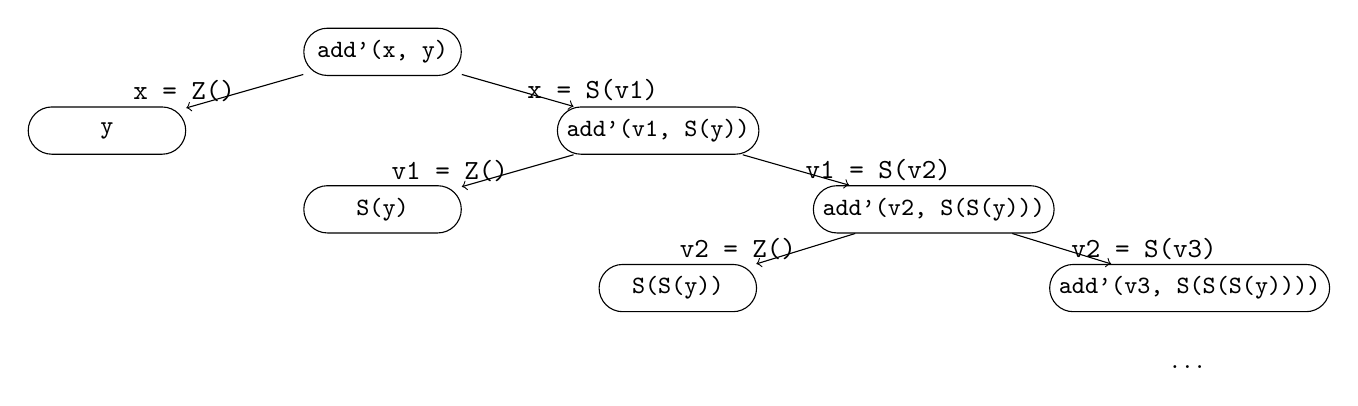
\begin{tikzpicture}[
level distance=10mm,
level/.style={sibling distance=40mm},
conf/.style={
	rectangle,minimum width=20mm,minimum height=6mm,rounded corners=3mm,
	draw=black,
	font=\ttfamily\small} 
]
\node[conf] {add'(x, y)} 
	child[->] {
		node[conf] {y}
		edge from parent node[left] {\texttt{x = Z()}}
	}
	child[->] {
		node[conf] {add'(v1, S(y))} 
		child[->] {
			node[conf] {S(y)}
			edge from parent node[left] {\texttt{v1 = Z()}}
		}
		child[->] {
			node[conf] {add'(v2, S(S(y)))} 
			child[->] {
				node[conf] {S(S(y))}
				edge from parent node[left] {\texttt{v2 = Z()}}
			}
			child[->] {
				node[conf] {add'(v3, S(S(S(y))))}
				child {node {\ldots} edge from parent[draw=none]}
				edge from parent node[right] {\texttt{v2 = S(v3)}}
			}
			edge from parent node[right] {\texttt{v1 = S(v2)}}
		}
		edge from parent node[right] {\texttt{x = S(v1)}}
	};
		
\end{tikzpicture}

This tree is not folding.
Indeed, a configuration can only be a renaming of another if both have the same size.
In this example, the path through the rightmost branches of the tree
contains ever-growing configurations.
However, if the size of configurations be bounded, the tree
will always fold to a finite graph.
%\footnote{
%Renaming gives rise in an obvious way to an equivalence relation,
%which partitions the set of expressions into equivalence classes.
%The set of SLL expressions containing constructors and functions only from a given
%program \texttt{p}, and with size limited from above, is thus partitioned
%into a finite number of equivalence classes.}.
\begin{exercise}
Try to prove the last statement. \textit{Hint:} To what kind of relation does
renaming naturally give rise?
\end{exercise}


We can thus apply a divide-and-conquer heuristics.
We limit the size of configurations inside nodes by some constant \texttt{sizeBound},
% дописать в духе: тогда их будет конечное число, т.к. конфигураций размера менее sizeBound - ограниченное
% (хоть и, возможно, экспоненциально большое - в этом одна из проблем суперкомпиляторов) количество.
and if the size of a configuration becomes larger than this constant,
we split it into smaller parts which we can process \emph{independently}.

Recall that the evaluation of closed SLL expressions is compositional.
For a closed expression $e_1 / \{v := e_2\}$ we have:
\[\mathcal{I}_p\llbracket e_1 / \{v := e_2\}\rrbracket = \mathcal{I}_p \llbracket e_1 / \{v := \mathcal{I}_p\llbracket e_2\rrbracket\} \rrbracket\]
The same property of compositionality holds for evaluation of tree of configurations.
(Look into SC~Mini source code to see how \texttt{intTree} handles splitted configurations.)


% немного запутанно; мне кажется, можно это более понятно нарисовать.
% как-то типа (картинка типа dot):
% f(e1,e2) -> f(e1,v)
% f(e1,e2) -> e2
% f(e1,v) ~~> c1 (содержит переменную v)
% e2 ~~> c2
% c1 -> c1[v:=c2]
% c2 -> c1[v:=c2]
% c1[v:=c2] ~~> value
% f(e1,e2) ~~> value
%
% и кстати, хорошо бы заметить, что это работает благодаря конфлюэнтности
% лямбда-исчисления, если я правильно понимаю (независимость от порядка редукций)

% еще вопрос: казалось бы, e[x:=y] это то же самое, что (\x -> e) y - зачем нужна
% специальная конструкция let? затем, что ее суперкомпилятор не "инлайнит", в отличие
% от вызовов безразличных функций?

SC~Mini limits the size of configurations in the tree and builds a foldable tree in the following way:
%\EZY{this sentence is too long, split it up}
\begin{itemize}
\item if while building the tree a configuration $e$ is encountered,
which is a function call, and whose size is greater than \texttt{sizeBound}, then
this configuration is splitted,
\item otherwise, the construction of the tree is done in the standard way.
\end{itemize}

Splitting represents the configuration $e$ as $e = e_1 / (v := e_2)$,
where $e_2$ is the largest subexpression of $e$, and $e_1$~--
the original expression $e$, in which $e_2$ is replaced by a (fresh) variable $v$.
Such configurations are encoded as \texttt{let}-expressions $let\;v = e_2 \;in \;e_1$.
%\footnote{
%The construction \texttt{let v = e2 in e1} plays in this case the technical role of
%a marker indicating that substitution must be postponed during reduction,
%and the machine $\mathcal{M}_p$ must produce as next steps 
%\texttt{e1} and \texttt{e2}, instead of \texttt{e1 / (v := e2)}.}. 
Then we process the configurations $e_1$ and $e_2$ independently.

\begin{exercise}
We do not need to check the size of constructor nodes. Why?
\end{exercise}

The configuration $e_1$ is a generalization of $e$. 
And $e$ is, in turn, a special instance of $e_1$.
By a slight abuse of terminology, the process of transforming the
tree of configurations into a foldable one -- as described above --
is also called \emph{generalization}.

Now, if we limit the growth of configurations (by size),
for any task we can build a (potentially infinite) tree of configurations,
which will in all cases be folded into a \emph{finite} graph of configurations.
Returning to our current example, if we set \texttt{sizeBound} equal to 5, then as
a result of generalizing the rightmost configuration we obtain:\\
\begin{tikzpicture}[
level distance=10mm,
level/.style={sibling distance=35mm},
conf/.style={
	rectangle,minimum width=20mm,minimum height=6mm,rounded corners=3mm,
	draw=black,
	font=\ttfamily\small},
comp/.style={
	font=\ttfamily\small
} 
]	 
\node[conf](base){add'(x, y)}
	child[->] {
		node[conf] {y}
		edge from parent node[left] {\texttt{x = Z()}}
	}
	child[->] {
		node[conf] {add'(v1, S(y))} 
		child[->] {
			node[conf] {S(y)}
			edge from parent node[left] {\texttt{v1 = Z()}}
		}
		child[->] {
			node[conf] {add'(v2, S(S(y)))} 
			child[->] {
				node[conf](b) {S(S(y))}
				edge from parent node[left] {\texttt{v2 = Z()}}
			}
			child[->] {
				node[conf,text width=25mm](let) {}
				child {node[conf](c1) {S(S(S(y)))} edge from parent[draw=none]}
				child {node[conf](c2) {add'(v3, v4)} edge from parent[draw=none]}
				edge from parent node[right] {\texttt{v2 = S(v3)}}
			}
			edge from parent node[right] {\texttt{v1 = S(v2)}}
		}
		edge from parent node[right] {\texttt{x = S(v1)}}
	};

%\node[conf](xxx) at (ggg) {xxx};	
\matrix [column sep=0pt] at (let) {
\node[comp]{let v4 =};&\node(v4)[token]{};&\node[comp]{in};&\node(in)[token]{}; \\ 
};
\draw [-] (v4.south) -- (c1.north);
\draw [-] (in.south) -- (c2.north);
\draw [->,dashed,rounded corners = 30pt] 
(c2.east) -- ($ (c2.east) + (20mm,0) $) -- ($ (base.east) + (20mm,0) $) -- (base.east);
\end{tikzpicture}

\begin{exercise} 
What properties should a task have, in order for the configuration
tree to be foldable without using generalization?
\end{exercise}

\begin{exercise}
It is very easy to extend \texttt{intTree} with treatment of \texttt{let}-expressions.
Check how it is done in the SC~Mini sources.
\end{exercise}

The idea of generalizing configurations is one of the cornerstones of supercompilation.
What we have described above is one of the possibly simplest and 
least sophisticated ways to perform generalization.

The supercompiler part responsible for deciding when to generalize is
historically called the \emph{whistle}.
Whistles in most existing supercompilers are typically more complicated
than just limiting configuration size.

The term ``whistle'', despite sounding a bit unscientific, is generally accepted
and used in most descriptions of supercompilation.
The whistle is a heuristic component, whose task is to signal the danger of
possibly non-foldable (and thus infinite) fragments appearing in the tree of configurations.
Of course, this task is an instance of the halting problem
(if the object language is Turing-complete) and does not have an exact solution.
Any whistle will necessarily give only approximative results, and even the
best heuristics cannot guarantee the absence of blunders, such as
whistling just a few steps before an actually foldable configuration.
The only strict requirement is to always err on the side of caution
and never let infinite tree paths slip through, as it would make
the supercompiler itself loop.

\subsection{Supercompiler prototype}

In the SC~Mini sources generalization and folding are implemented via following functions:
\begin{itemize}
\item \texttt{buildFTree} -- it builds a foldable tree of configurations by limiting size of configurations
(by means of splitting)
\item \texttt{foldTree} -- it takes a (possibly infinite) tree of configurations and folds it into a finite graph.
\end{itemize}

Let's create the following program transformer:
\begin{lstlisting}[language=haskell]
transform :: Task -> Task
transform (e, p) =
	residuate $ foldTree $ buildFTree (driveMachine p) e
\end{lstlisting}

A most interesting thing in this transformer happens there:
the machine $\mathcal{M}_p$ is not only run -- the result of its run
is analyzed, and possibly a decision to generalize is taken.

We argue that this program transformer fulfills the requirements of the
previously stated definition of ``supercompiler''.
Although this transformer performs no interesting optimizations, it
can serve as a foundation for a full-blown supercompiler.
We shall use it as a baseline to which we shall compare the
transformers that follow (deforestation and supercompilation).

\begin{exercise}
Try to show that for each task \texttt{(e, p)} and each substitution
\texttt{s} the computation \texttt{sll\_run (e', p') s} (where \texttt{(e', p')}
is the corresponding residual task) requires exactly as many reduction steps
as the computation \texttt{sll\_run (e, p) s}. 
That means that the transformer \texttt{transform} does not degrade performance,
but it does not improve it either.
\end{exercise}

Does this transformer modify the input program at all? Yes, and here is an example:
%\footnote{
%The residual program is listed here exactly as produced by \texttt{transform}.
%There are fresh function names based on an increasing counter.
%Of course, it would be nice to generate more meaningful names for the
%newly created functions, but -- while feasible -- 
%it is outside the scope of our toy supercompiler.}:
% Если хватит сил, можно подписать в виде комментариев ``старые'' выражения.
\begin{lstlisting}[language=sll,escapechar=!]
(even(sqr(x)), prog1) !$\xRightarrow{transform}$! (f1(x), prog1T)
\end{lstlisting}
Where \texttt{prog1T =}
\begin{lstlisting}[language=sll]
f1(x) = g2(x, x);
g2(Z(), x) = f3();
g2(S(v1), x) = g4(x, x, v1);
f3() = True();
g4(Z(), x, v1) = g5(v1, x);
g4(S(v2), x, v1) = f7(v2, v1, x);
g5(Z(), x) = f6();
g5(S(v2), x) = g4(x, x, v2);
f6() = True();
f7(v2, v1, x) = g8(v2, v1, x);
g8(Z(), v1, x) = g9(v1, x);
g8(S(v3), v1, x) = f16(v3, v1, x);
g9(Z(), x) = f10();
g9(S(v3), x) = g11(x, x, v3);
f10() = False();
g11(Z(), x, v3) = g9(v3, x);
g11(S(v4), x, v3) = f12(v4, v3, x);
f12(v4, v3, x) = g13(v4, v3, x);
g13(Z(), v3, x) = g14(v3, x);
g13(S(v5), v3, x) = f7(v5, v3, x);
g14(Z(), x) = f15();
g14(S(v5), x) = g4(x, x, v5);
f15() = True();
f16(v3, v1, x) = g17(v3, v1, x);
g17(Z(), v1, x) = g18(v1, x);
g17(S(v4), v1, x) = f7(v4, v1, x);
g18(Z(), x) = f19();
g18(S(v4), x) = g4(x, x, v4);
f19() = True();
\end{lstlisting}

We can easily detect at least one property of the transformer -- the resulting program
contains no nested function calls: it is ``flat''.
%\footnote{
%This program is clearly more machine-oriented -- easier to execute or analyze 
%by computer, but harder to understand by humans (could you guess
%its purpose at first glance?).}.

\subsection{KMP Test}

\begin{figure}[t!]
\caption{\texttt{prog2}: find a substring inside a string}
\label{fig:prog2}
\begin{lstlisting}[language=sll]
match(p, s) = m(p, s, p, s);

-- matching routine
-- current pattern is empty, so match succeeds
m("", ss, op, os) = True();
-- proceed to match first symbol of pattern
m(p:pp, ss, op, os) = x(ss, p, pp, op, os);

-- matching of the first symbol
-- current string is empty, so match fails
x("", p, pp, op, os) = False();
-- compare first symbol of pattern with first symbol of string
x(s:ss, p, pp, op, os) =
  if(eq(p, s), m(pp, ss, op, os), n(os, op));

-- failover
-- current string is empty, so match fails
n("", op) = False();
-- trying the rest of the string
n(s:ss, op) = m(op, ss, op, ss);

-- equality routines
eq('A', y) = eqA(y);  eqA('A') = True();   eqB('A') = False();
eq('B', y) = eqB(y);  eqA('B') = False();  eqB('B') = True();
-- if/else
if(True(), x, y) = x;
if(False(), x, y) = y;
\end{lstlisting}
\end{figure}

Consider the program in Fig.~\ref{fig:prog2}
(where function names are deliberately short, to keep the drawings of graphs of configurations
small):
the function \texttt{match(p, s)} checks if a string \texttt{p}
is contained inside the string \texttt{s}.
For simplicity we use a 2-letter alphabet -- \texttt{`A'} and \texttt{`B'}.
Strings are represented -- as in Haskell -- by lists of characters.
We also use some list/string syntactic sugar from
Haskell for readability, even if it is not actually implemented in SLL.

The function \texttt{match} is general, but inefficient.
Consider the call \texttt{match("AAB", s)},
which checks if the substring (pattern) \texttt{"AAB"} appears inside the string \texttt{s}.
Our program will perform this check in the following way: compare \texttt{`A'}
with the first character of \texttt{s}, \texttt{`A'} -- with the second one,
\texttt{'B'} -- with the third one.
If any of these comparisons fails, we restart the comparison sequence
after skipping the first character of \texttt{s}.
This strategy is far from optimal, however.
Let's assume that the string \texttt{s} starts with \texttt{"AAA\ldots"}.
The first 2 comparisons will succeed, the 3rd one will fail.
It is inefficient to repeat the same sequence of comparisons
on the tail \texttt{"AA\ldots"},
as we already have enough information to know, that the first 2 comparisons of \texttt{"AAB"}
with \texttt{"AA\ldots"} will succeed.
The deterministic finite automaton (DFA), built by the Knuth-Morris-Pratt algorithm \cite{Knuth1977Fast},
will consider each character of \texttt{s} at most once.

A simple way to estimate the power of an optimizing transformation is to see if it
can produce -- fully automatically -- a well-known efficient algorithm
from a ``na\"{\i}ve'', less-efficient one.
In the case of supercompilation, it turns out that
-- starting from a na\"{\i}ve string-matching algorithm,
and fixing the value of the substring we try to match --
we can automatically obtain an efficient specialized matching program,
analogous in action to the well-known Knuth-Morris-Pratt algorithm
(hence the name of the test).

Our original simple transformer \texttt{transform} is unable to obtain an efficient matching program.
But in the next couple of sections, we will augment \texttt{transform} using two ``tricks'',
which are key ingredients of ``real'' supercompilers, and the transformer \texttt{supercompile} produces
a residual task exactly corresponding to this DFA.

This program is the so-called KMP-test, which is
a classical example in the context of supercompilation, as it demonstrates its greater
power compared to similar program transformations like deforestation and partial
evaluation\cite{Sorensen1994TurchinSupercompiler,Sorensen1998Introduction}.
This test is not only a good demonstration of the combined effect of the two tricks mentioned above,
but it also gives some measure of the extent of program transformations performed by supercompilation.

% подчеркнуть, что КМП в общем виде - не выводится, выводится лишь его экземпляр для конкретного
% паттерна (кстати интересно, есть ли суперкомпиляторы, которые могут вывести КМП в общем виде?).

Our original simple transformer \texttt{transform} gives the following result:
\begin{lstlisting}[language=sll,escapechar=!]
(match("AAB", s), prog2) !$\xRightarrow{transform}$! (f1(s), prog2T)
\end{lstlisting}
where \texttt{prog2T} is:
% если будут силы, подпишем в виде комментариев старые выражения
\begin{lstlisting}[language=sll]
f1(s) = f2(s);
f2(s) = g3(s, s);
g3("", s) = False();
g3(v1:v2, s) = f4(v1, v2, s);
f4(v1, v2, s) = g5(v1, v2, s);
g5('A', v2, s) = f6(v2, s);
g5('B', v2, s) = f22(v2, s);
f6(v2, s) = f7(v2, s);
f7(v2, s) = g8(v2, s);
g8("", s) = False();
g8(v3:v4, s) = f9(v3, v4, s);
f9(v3, v4, s) = g10(v3, v4, s);
g10('A', v4, s) = f11(v4, s);
g10('B', v4, s) = f20(v4, s);
f11(v4, s) = f12(v4, s);
f12(v4, s) = g13(v4, s);
g13("", s) = False();
g13(v5:v6, s) = f14(v5, v6, s);
f14(v5, v6, s) = g15(v5, v6, s);
g15('A', v6, s) = f16(v6, s);
g15('B', v6, s) = f18(v6, s);
f16(v6, s) = g17(s);
g17("") = False();
g17(v7:v8) = f2(v8);
f18(v6, s) = f19(v6, s);
f19(v6, s) = True();
f20(v4, s) = g21(s);
g21("") = False();
g21(v5:v6) = f2(v6);
f22(v2, s) = g23(s);
g23("") = False();
g23(v3:v4) = f2(v4);
\end{lstlisting}
% можно ли этой программе дать human-readable названия функций? а то совсем ничего непонятно,
% неясна механика ее работы и неясно, что же сделал суперкомпилятор.
This long listing is reproduced here only to serve as a baseline for comparison.
Note that the residual program contains no nested function calls,
but each of the characters of \texttt{s} may be checked multiple times, as in the input program.

\subsection{Transient step removal}

Very often graphs of configurations contain fragments of the following kind:
\begin{lstlisting}[language=haskell,escapechar=!]
... c1 !$\rightarrow$! c2 !$\rightarrow$! c3 ...
\end{lstlisting}
where the transition \texttt{c2 $\rightarrow$ c3} corresponds to a transient step 
(as defined in subsection ``Driving'').
We can always -- thanks to the absence of side effects in SLL -- replace such a fragment by:
\begin{lstlisting}[language=haskell,escapechar=!]
... c1 !$\rightarrow$! c3 ...
\end{lstlisting}
% указать, что это практически inlining

As an example, consider the top part of the graph of configurations 
for the KMP-test program, which is produced by 
\texttt{transform}:\\
\begin{tikzpicture}[
level distance=12mm,
level/.style={sibling distance=35mm},
conf/.style={
	rectangle,minimum width=20mm,minimum height=6mm,rounded corners=3mm,
	draw=black,
	font=\ttfamily\small} 
]
\tikzstyle{level 3}=[sibling distance=65mm]
\tikzstyle{level 5}=[sibling distance=40mm]
\node[conf](x1){match("AAB", s)}
child[->,decorate,decoration=snake] {node[conf](b) {m("AAB", s, "AAB", s)} 
	child[->] {node[conf] {x(s, 'A', "AB", "AAB", s)} 
		child[->] {node[conf] {False()}
			edge from parent node[left] {\texttt{s = ""}}}
		child[->] {node[conf]{if(eq('A', v1), m("AB", v2, "AAB", s), n(s, "AAB"))}
			child[->]{node[conf] {if(eqA(v1), m("AB"), v2, "AAB", s), n(s, "AAB"))}
				child[->] {node[conf,xshift=-30mm] {\ldots}
					edge from parent node[left] {\texttt{v1 = 'A'}}
				}
				child[->] {node[conf,xshift=-5mm]{if(False(), m("AB", v2, "AAB", s), n(s, "AAB"))}
					child[->]{
						node[conf] {n(s, "AAB")}
						child[->] {node[conf] {False}
							edge from parent node[left] {\texttt{s = ""}}}
						child[->] {node[conf](a) {m("AAB", v4, "AAB", v4)}
							edge from parent node[right] {\texttt{s = v3:v4}}}
						edge from parent[->,decorate,decoration=zigzag]}
					edge from parent node[right] {\texttt{v1 = 'B'}}
				}
				edge from parent[->,decorate,decoration=zigzag]
				}
				edge from parent node[right] {\texttt{s = v1:v2}}}}
edge from parent[->,decorate,decoration=zigzag]
};
\draw [->,dashed,rounded corners = 10pt] 
(a.east) -- ($ (a.east) + (15mm,0) $) -- ($ (b.east) + (65mm,0) $) -- (b.east);
\end{tikzpicture}\\
% можно ли в этих всех картинках использовать синтаксис Cons(v1,v2) вместо v1:v2?
% поскольку он используется в текстах на SLL.
The transient steps are displayed with zigzag arrows.
If we remove them, the cleaned-up graph of configurations will look like this:\\
\begin{tikzpicture}[
level distance=12mm,
level/.style={sibling distance=35mm},
conf/.style={
	rectangle,minimum width=20mm,minimum height=6mm,rounded corners=3mm,
	draw=black,
	font=\ttfamily\small} 
]
\tikzstyle{level 2}=[sibling distance=65mm]
\node[conf](b) {m("AAB", s, "AAB", s)} 
	child[->] {node[conf] {x(s, 'A', "AB", "AAB", s)} 
		child[->] {node[conf] {False()}
			edge from parent node[left] {\texttt{s = ""}}}
		child[->] {node[conf] {if(eqA(v1), m("AB", v2, "AAB", s), n(s, "AAB"))}
			child[->] {node[conf,xshift=-10mm] {\ldots}
				edge from parent node[left] {\texttt{v1 = 'A'}}
			}
			child[->] {node[conf,xshift=-10mm] {n(s, "AAB")}
				child[->] {node[conf] {False}
					edge from parent node[left] {\texttt{s = ""}}}
				child[->] {node[conf](a) {m("AAB", v4, "AAB", v4)}
					edge from parent node[right] {\texttt{s = v3:v4}}}
				edge from parent node[right] {\texttt{v1 = 'B'}}
			}
			edge from parent node[right] {\texttt{s = v1:v2}}}};
\draw [->,dashed,rounded corners = 10pt] 
(a.east) -- ($ (a.east) + (20mm,0) $) -- ($ (b.east) + (50mm,0) $) -- (b.east);
\end{tikzpicture}

The SC~Mini sources contain a transformer \texttt{deforest} -- a modification
of \texttt{transform} -- which removes transient edges and the corresponding nodes
from the graph of configurations.

If we pass the test program through \texttt{deforest}, we get:
% кратко пояснить, что это такое (дефорестатор)
\begin{lstlisting}[language=sll,escapechar=!]
(match("AAB", s), prog2) !$\xRightarrow{deforest}$! (f1(s), prog2D)
\end{lstlisting}
where \texttt{prog2D = }
% аналогично, здесь бы human-readable имена функций
\begin{lstlisting}[language=sll]
f1(s) = g2(s, s);
g2("", s) = False();
g2(v1:v2, s) = g3(v1, v2, s);
g3('A', v2, s) = g4(v2, s);
g3('B', v2, s) = g10(s);
g4("", s) = False();
g4(v3:v4, s) = g5(v3, v4, s);
g5('A', v4, s) = g6(v4, s);
g5('B', v4, s) = g9(s);
g6("", s) = False();
g6(v5:v6, s) = g7(v5, v6, s);
g7('A', v6, s) = g8(s);
g7('B', v6, s) = True();
g8("") = False();
g8(v7:v8) = f1(v8);
g9("") = False();
g9(v5:v6) = f1(v6);
g10("") = False();
g10(v3:v4) = f1(v4);
\end{lstlisting}

The deforested program contains less than half the number of functions (23 vs. 10)
compared to the result of \texttt{transform},
as some intermediate functions were removed (roughly speaking, inlined).
Although the residual program is smaller, it still contains the same inefficiency 
we discussed above.

The removal of transient edges is a form of simplification of graphs of configurations.
This simplification is \emph{one of the two} main mechanisms for optimization,
which are employed by supercompilation. 
It is most effective when used in conjunction with the second mechanism
-- information propagation -- which we shall discuss next.

\begin{exercise}
It is also possible to remove transient steps from the tree of configurations (before folding it to a graph).
What pitfalls might such an approach have?
\end{exercise}
% Ответ: возможно зацикливание. Например f(x) = f(f(x)) - одни транзитные шаги.

%\subsubsection{Interlude: deforestation}

There is a separate program transformation technique 
called \emph{deforestation}~\cite{Wadler1988deforestation,Ferguson1988When}.
Its main goal is to reduce the creation of intermediate data structures
-- lists, trees (hence the name), etc. -- which arise as a result of
composing different functions in a program.
Ferguson et al.~\cite{Ferguson1988When} describe deforestation for a language
very similar to SLL\@.
Classical deforestation does not require generalization, as it considers
only programs conforming to certain syntactic restrictions
(which guarantee that the resulting tree is always foldable).
A practical advantage of deforestation is that for
many special cases it can be formulated as a simple set of
rewrite rules (\emph{shortcut deforestation}, or \emph{shortcut fusion}~-- 
see for example \cite{gill1993scd}), which are easy to implement. 
A form of shortcut deforestation is implemented inside GHC, for example.

\subsection{Information propagation}

Here is the graph of configurations for the KMP test produced by \texttt{deforest}:\\
\begin{tikzpicture}[
level distance=12mm,
level/.style={sibling distance=35mm},
conf/.style={
	rectangle,minimum width=20mm,minimum height=6mm,rounded corners=3mm,
	draw=black,
	font=\ttfamily\small}
]
\tikzstyle{level 2}=[sibling distance=65mm]
\node[conf](b) {m("AAB", s, "AAB", s)}
	child[->] {node[conf] {x(s, 'A', "AB", "AAB", s)}
		child[->] {node[conf] {False()}
			edge from parent node[left] {\underline{\texttt{s = ""}}}}
		child[->] {node[conf] {if(eqA(v1), m("AB", v2, "AAB", s), n(s, "AAB"))}
			child[->] {node[conf,xshift=-10mm] {\ldots}
				edge from parent node[left] {\texttt{v1 = 'A'}}
			}
			child[->] {node[conf,xshift=-10mm] {n(s, "AAB")}
				child[->] {node[conf] {False}
					edge from parent node[left] {\underline{\underline{\texttt{s = ""}}}}}
				child[->] {node[conf](a) {m("AAB", v4, "AAB", v4)}
					edge from parent node[right] {\underline{\underline{\texttt{s = v3:v4}}}}}
				edge from parent node[right] {\texttt{v1 = 'B'}}
			}
			edge from parent node[right] {\underline{\texttt{s = v1:v2}}}}};
\draw [->,dashed,rounded corners = 10pt]
(a.east) -- ($ (a.east) + (20mm,0) $) -- ($ (b.east) + (50mm,0) $) -- (b.east);
\end{tikzpicture}

It contains a step which checks if the string \texttt{s} is empty or not (underlined).
Below it, there is another step, which makes the same check (double-underlined),
although we have assumed already that \texttt{s} is not empty 
(in the corresponding subtree after the first check). 
Such repeated checks are clearly redundant.

Supercompilers remove such redundancies as follows:
each time case analysis is performed during driving,
information about its outcome is propagated in each corresponding subtree.

Let's propagate the fact that \texttt{s = v1:v2} (and hence non-empty) in the corresponding subtree:\\
\begin{tikzpicture}[
level distance=12mm,
level/.style={sibling distance=35mm},
conf/.style={
	rectangle,minimum width=20mm,minimum height=6mm,rounded corners=3mm,
	draw=black,
	font=\ttfamily\small} 
]
\tikzstyle{level 2}=[sibling distance=70mm]
\node[conf](b) {m("AAB", s, "AAB", s)} 
	child[->] {node[conf] {x(s, 'A', "AB", "AAB", s)} 
		child[->] {node[conf] {False()}
			edge from parent node[left] {\texttt{s = ""}}}
		child[->] {node[conf] {if(eqA(v1), m("AB"), v2, "AAB", v1:v2), n(v1:v2, "AAB"))}
			child[->] {node[conf] {\ldots}
				edge from parent node[left] {\texttt{v1 = 'A'}}
			}
			child[->] {node[conf] {n('B':v2, "AAB")}
				child[->] {node[conf](a) {m("AAB", v2, "AAB", v2)}
					edge from parent[->,decorate,decoration=zigzag]
				}
				edge from parent node[right] {\texttt{v1 = 'B'}}
			}
			edge from parent node[right] {\texttt{s = v1:v2}}}};
\draw [->,dashed,rounded corners = 10pt] 
(a.east) -- ($ (a.east) + (20mm,0) $) -- ($ (b.east) + (70mm,0) $) -- (b.east);
\end{tikzpicture}\\
We have not only removed a superfluous test, but we have also unmasked
a transient step, which can be further removed.
As a result we obtain:\\
\begin{tikzpicture}[
level distance=12mm,
level/.style={sibling distance=35mm},
conf/.style={
	rectangle,minimum width=20mm,minimum height=6mm,rounded corners=3mm,
	draw=black,
	font=\ttfamily\small} 
]
\tikzstyle{level 2}=[sibling distance=70mm]
\node[conf](b) {m("AAB", s, "AAB", s)} 
	child[->] {node[conf] {x(s, 'A', "AB", "AAB", s)} 
		child[->] {node[conf] {False()}
			edge from parent node[left] {\texttt{s = ""}}}
		child[->] {node[conf] {if(eqA(v1), m("AB"), v2, "AAB", v1:v2), n(v1:v2, "AAB"))}
			child[->] {node[conf] {\ldots}
				edge from parent node[left] {\texttt{v1 = 'A'}}
			}
			child[->] {node[conf](a) {m("AAB", v2, "AAB", v2)}
				edge from parent node[right] {\texttt{v1 = 'B'}}
			}
			edge from parent node[right] {\texttt{s = v1:v2}}}};
\draw [->,dashed,rounded corners = 10pt] 
(a.east) -- ($ (a.east) + (25mm,0) $) -- ($ (b.east) + (65mm,0) $) -- (b.east);
\end{tikzpicture}

The transformer \texttt{supercompile} (inside SC~Mini sources) implements such information propagation.
In contrast to \texttt{deforest}, each time driving performs case analysis,
its results are propagated in the corresponding new configurations.
Recall that SLL contains just a single kind of test -- matching the first argument of 
a curious function against a list of simple patterns.
Hence, the only kind of information we can propagate is that
a given configuration variable is equal to a given pattern.
Such a (restricted) form of information propagation is 
called \emph{positive information propagation}.
Correspondingly, supercompilers propagating only positive informtion
are called \emph{positive supercompilers}.
If, for example, SLL permitted also default clauses
(in curious-function definitions), we could propagate 
also negative information -- in the default clause -- that
the variable is not equal to any of the patterns in the list.
A supercompiler, which propagates both positive and negative information,
is called \emph{perfect} \cite{Secher2000Perfect}. It is also possible to have intermediate 
situations, where only some forms of negative information are propagated.
% хорошо бы пример, когда это могло бы что-то дать. мне сходу не удалось его мысленно построить.

Here is the final result of supercompiling our KMP test:
% human-readabilize
\begin{lstlisting}[language=sll,escapechar=!]
(match("AAB", s), prog2) !$\xRightarrow{supercompile}$! (f1(s), prog2S)
\end{lstlisting}
where \texttt{prog2S = }
\begin{lstlisting}[language=sll]
f1(s) = g2(s);
g2("") = False();
g2(v1:v2) = g3(v1, v2);
g3('A', v2) = g4(v2);
g3('B', v2) = f1(v2);
g4("") = False();
g4(v3:v4) = g5(v3, v4);
g5('A', v4) = f6(v4);
g5('B', v4) = f1(v4);
f6(v4) = g7(v4);
g7("") = False();
g7(v5:v6) = g8(v5, v6);
g8('A', v6) = f6(v6);
g8('B', v6) = True();
\end{lstlisting}

We finally obtain the desired effect: each character of the string \texttt{s}
is considered at most once.

\begin{exercise}
Prove the last statement.
\end{exercise}

The information propagation we have just described is the second optimization mechanism 
employed by supercompilation (the first was the removal of transient steps).
This propagation has 3 important effects:
\begin{enumerate}
  \item No variable is tested twice.
  \item Avoiding repeated tests uncovers further possibilities for removing transient steps.
  \item The graph of configurations is pruned of unreachable branches, which results in dead-code 
  removal in the residual program.
\end{enumerate}
In the example above, the graph built by \texttt{deforest} contains the following path:
\begin{lstlisting}[language=sll,escapechar=!]
{s = v1:v2}  !$\rightarrow$! ... !$\rightarrow$! {s = ""} !$\rightarrow$!
\end{lstlisting}
It is clear that no actual computation can take this path. 
Deforestation, however, leaves it in the residual program;
as a result the deforested program \texttt{prog2d} above contains a function
\texttt{g10} whose first argument can never be an empty string:
\begin{lstlisting}[language=sll]
g10("") = False();
g10(v3:v4) = f1(v4);
\end{lstlisting}

As a result of supercompiling the KMP test, we obtained a program which contains no dead code.
Of course, this is not always possible, as dead-code removal is undecidable in general.
In the case of supercompilation, dead code may still appear in the residual program
if we have applied generalization.

\begin{exercise}
Most works discussing supercompilation interweave information propagation with other
aspects of the transformation (for example, with transient-step removal).
Check if this is the case as well inside SC~Mini's sources.
%В большинстве работ по суперкомпиляции распространение информации рассматривается как обязательная
%операция. В SC Mini распространение информации выделено как отдельный логический шаг~-- модификация машины
%$\mathcal{M}_p$:
%\\
%\texttt{addPropagation :: Machine Conf $\rightarrow$ Machine Conf}
\end{exercise}

\subsection{The essence of SC Mini}

This section turned out rather long, so let's take a brief look -- from 
a slightly different angle -- at what it covered.

The SC~Mini supercompiler is an attempt to build a minimalistic supercompiler in Haskell.
Its main goal is to delineate the main ingredients which are present in most supercompilers
and show how they can be combined to work well together.

Let's review the gradual transition from the basic transformer \texttt{transform}
(which neither improves, nor degrades performance), passing through \texttt{deforest},
and finally arriving at the ultimate transformer \texttt{supercompile}.

\noindent Starting from the baseline transformer \texttt{transform}\ldots
\begin{lstlisting}[escapechar=!]
transform :: Task -> Task
transform (e, p) =
    residuate $ foldTree $
        buildFTree (driveMachine p) e
\end{lstlisting}
% пояснить бы, что buildFTree делает, а также drive и propagate drive, хотя бы концептуально.
% (пояснить, что buildFTree прогоняет с помощью произвольной стратегии прогонки - либо с
% распространением, либо без; и что любую стратегию прогонки можно дополнить распространением
% информации - поэтому propagate это HOF)
\ldots we add simplification of the graph of configurations by removing transient steps\ldots
\begin{lstlisting}[escapechar=!]
deforest :: Task -> Task
deforest (e, p) =
    residuate $ !\underline{simplify}! $ foldTree $
        buildFTree (driveMachine p) e
\end{lstlisting}
\ldots and we finish by adding information propagation:
\begin{lstlisting}[escapechar=!]
supercompile :: Task -> Task
supercompile (e, p) =
    residuate $ !\underline{simplify}! $ foldTree $
        buildFTree (!\underline{addPropagation}!  $ driveMachine p) e
\end{lstlisting}

Thanks to propagating test outcomes in the corresponding consequent configurations
and further simplifications of the graph, our minimalistic supercompiler
managed to convert a na\"{\i}ve substring search algorithm into the well-known
efficient KMP algorithm.

\subsection{Not only optimization}

% \begin{figure}[t]
% \caption{\texttt{prog3}}
% \label{fig:prog3}
% \begin{lstlisting}[language=sll]
add(Z(), y) = y;
add(S(x), y) = S(add(x, y));

double(Z()) = Z();
double(S(x)) = S(S(double(x)));

half(Z()) = Z();
half(S(x)) = half1(x);
half1(Z()) = Z();
half1(S(x)) = S(half(x));

eq(Z(), y) = eqZ(y);
eq(S(x), y) = eqS(y, x);
eqZ(Z()) = True();
eqZ(S(x)) = False();
eqS(Z(), x) = False();
eqS(S(y), x) = eq(x, y);
\end{lstlisting}
% \end{figure}

% Рассмотрим
% программу \texttt{prog3} (Рис.~\ref{fig:prog3}). Можно по индукции (рассматривая все правила
% операционной семантики SLL) доказать утвержение, что для любого \texttt{n}:
% \texttt{half(double(n))~==~n}.
%
% Данное утверждение может быть доказано, если рассмотреть выражение \texttt{eq(half(double(n)), n)} и
% показать, что результатом его вычисления может быть только \texttt{True()}\footnote{Предварительно
% согласившись, что \texttt{eq} кодирует ``равенство'' результатов.}.
% \begin{lstlisting}[language=sll,escapechar=!]
% (eq(half(double(n)), n), prog3) !$\xRightarrow{supercompile}$! (g1(n), prog3S)
% \end{lstlisting}
% где \texttt{prog3S}:
% \begin{lstlisting}[language=sll]
% g1(Z()) = True(); g1(S(v1)) = g1(v1);
% \end{lstlisting}

SC Mini can also be used to check different program properties.
Let's show that the operation \texttt{add} -- defined in \texttt{prog1} --
is associative, that is, for all arguments \texttt{args}:
\begin{lstlisting}
sll_run (add(add(x,y),z), p1) == sll_run (add(x,add(y,z), p1)
\end{lstlisting}
We could of course prove this by induction (using the rules of SLL operational semantics).
But we can also compare the residual programs produced by SC~Mini in both cases --
they turn out syntactically equivalent:
\begin{lstlisting}[language=sll,escapechar=!]
(add(add(x, y), z), p1) !$\xRightarrow{supercompile}$! (g1(x, y, z), prog3S')
(add(x, add(y, z)), p1) !$\xRightarrow{supercompile}$! (g1(x, y, z), prog3S')
\end{lstlisting}
where \texttt{prog3S' =}
\begin{lstlisting}[language=sll]
g1(Z(), y, z) = g2(y, z);
g1(S(v1), y, z) = S(g1(v1, y, z));
g2(Z(), z) = z;
g2(S(v1), z) = S(g2(v1, z));
\end{lstlisting}
This is enough to prove associativity of \texttt{add} (assuming of course
that SC~Mini always preserves the semantics of the input program), as we have:
\begin{lstlisting}
sll_run (add(add(x, y), z), p1) ==
  sll_run (g1(x, y, z), prog3S') ==
    sll_run (add(x, add(y, z)), p1)
\end{lstlisting}
